\chapter{Second-Order System Identification and Analysis}\label{Lab:2}
A large majority of systems we wish to control are physical systems. These
systems are often modelled using Newton's laws
\[
\begin{aligned}
  \mathrm{mass}~\frac{\mathrm d}{\mathrm{d}t}~\mathrm{position}
    &= \sum \mathrm{natural~forces} + \mathrm{applied~force},\\
  \mathrm{inertia}~\frac{\mathrm d}{\mathrm{d}t}~\mathrm{orientation}
    &= \sum \mathrm{natural~torques} + \mathrm{applied~torque},
\end{aligned}
\]
which result in second-order differential equations. These systems --- when
they are linear --- result in second-order transfer functions from the
applied input (forces or torques) to the output (position and orientation).
In other words, if we want to know how to effectively control physical systems,
we must first understand second-order systems and their properties!

In this lab you will explore the generic characteristics of a second-order
linear system. More fundamentally, you will realize the value of learning
control theory. You will discover the limitations of proportional error
feedback control --- the most na\'ive of control laws --- when applied to
a physical system. This hopefully motivates you to explore why we consider
more complicated control strategies. Lab~\ref{Lab:4} further expands on this
idea by exploring PID control.

\section{Objectives}
The primary objectives of this lab are to
\begin{enumerate}[label=(\arabic*)]
  \item{
    \textbf{Learn} the characteristic properties of a second-order linear
    system.
  }
  \item{
    \textbf{Identify} the parameters of a second-order linear system.
  }
  \item{
    \textbf{Learn} how to acquire a Bode plot, the frequency response,
    and \textbf{understand} how to interpret it.
  }
  \item{
    \textbf{Explore} how a proportional control feedback affects the response
    of a second-order system.
  }
\end{enumerate}
Like Lab~\ref{Lab:1}, this is not a long lab.

\section{Experimental Procedure}
This entire lab will be done using the ``\texttt{Lab\_2.slx}'' Simulink model.
In there you will
find a number of blocks already placed for you in an open loop configuration:
\begin{itemize}
  \item{a signal generator,}
  \item{a summing junction,}
  \item{an adjustable gain block,}
  \item{a ``fill-in'' disturbance block,}
  \item{a ``plant'', the system we are going to analyze, and}
  \item{a terminator.}
\end{itemize}
This time, we will \emph{not} use the signal generator and instead leverage
the Model Linearizer App. Its usage is described in Appendix
\ref{App:Simulink:ModelLinearizer}. You may acquire the step response
using the techniques described in Lab~\ref{Lab:1} but to acquire the frequency
response you will have to use the Model Linearizer app. In future, I advise
you to use the Model Linearizer app, as it'll unify all your data collection
requirements and is far easier to use than modifying a script and turning
on/off logging. For this lab, the input signal starts off configured
as \(r\) and the output signal as \(y.\) You will have to change it later
in the lab.
%
The plant --- labelled \(P(s)\) in the Simulink diagram --- can be assumed
to be a transfer function taking the form
\[
  P(s) = \frac{K}{s^2 + a s + b},
\]
where \(a, b, K > 0.\) Equivalently, we can express \(P(s)\) in what is known
as the standard second order form
\[
  P(s) = \frac{\hat{K} \omega^2}{s^2 + 2 \zeta \omega s + \omega^2}.
\]
The primary goal of this experiment is to explore
the characteristics of your system as well as how it changes as we
affect a proportional error gain.

\subsection{Measuring the Characteristics of a Second Order System}
In Lab~\ref{Lab:1}, you learned about the DC gain, the bandwidth, and
settling time of a first-order system.
We will once gain acquire the DC gain, bandwidth and settling times
whose definition does not change when applied to a second-order system.

However, there are a few more characteristics we would like to identify.
The first notion is that of the overshoot. There are a variety of ways
to define the overshoot. For us, the following definition suffices.
%
\begin{definition}[]{Time-To-Peak and Overshoot}
  Let \(G(s)\) be a proper, stable transfer function
  that maps an input signal \(u(t)\) to an output \(y(t).\)
%
  Let \(u(t)\) be the (not necessarily unit) step function. The peak value
  of \(y(t)\) is the maximum value \(y(t)\) obtains, mathematically expressed
  by
  \[
    y_\mathrm{max} \defineas \max_{\tau \in \Real} \left| y(\tau) \right|
  \]
  and the time it obtains the peak value, known as \textbf{time-to-peak}
  is defined as
  \[
    T_\mathrm{peak} \defineas \argmax_{\tau \in \Real} \left| y(\tau) \right|.
  \]
  Then, if \(y_\mathrm{ss}\) is the steady-state value of \(y(t),\) the
  \textbf{percent overshoot} is defined as
  \[
    \%\mathrm{OS}
      \defineas
        \frac{\left| y_\mathrm{max} - y_\mathrm{ss} \right|}{y_\mathrm{ss}}.
  \]
\end{definition}
%
\begin{figure}
  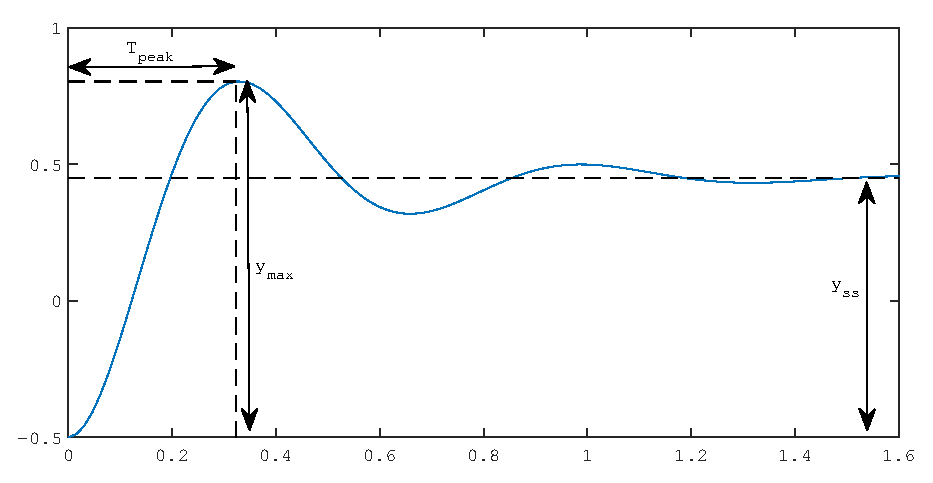
\includegraphics{images/Lab_2_Peak.eps}
  \caption[Depicting Overshoot Measurements for a Second-Order System.]{%
    The maximum peak occurs at time \(T_\mathrm{peak}\) with amplitude
    \(y_\mathrm{max}.\) The steady-state value is shown as \(y_{\mathrm{ss}}.\)
  }
  \label{fig:lab2:peak}
\end{figure}
%
Figure~\ref{fig:lab2:peak} depicts the measurements you will perform to acquire
the percent overshoot. You measure the maximum value of the output
signal and the settling value of the signal. Then you
compute the relative error between the maximum value and the settling value of
the output. The time-to-peak value is another characteristic constant we
measure.
%
\begin{procedure}[label={proc:lab2:p1}]
  In this procedure you will capture a variety of characteristics of
  your provided second-order system.
  \begin{enumerate}[label=(\arabic*)]
    \item{
      \textbf{Ensure} your system is in the open loop configuration.
    }
    \item{
      \textbf{Ensure} that you indicate the signal before the summing junction
      is an input signal (Input Perturbation) and the signal after the plant
      is indicated as an output signal (Output Measurement). Refer
      to Appendix~\ref{App:Simulink:ModelLinearizer:2} for more information
      on how to do so.
    }
    \item{
      \textbf{Open} the Model Linearizer app and \textbf{capture} a
      step response. Refer to Appendix~\ref{App:Simulink:ModelLinearizer:3}
      on how to do so.
    }
    \item{
      \textbf{Measure} and \textbf{record} the following parameters of the
      output signal:
      \begin{itemize}
        \item{
          the steady-state value \(y_{\mathrm{ss}},\)
        }
        \item{
          the time-to-peak value \(T_{\mathrm{peak}}\) and
          the peak value \(y_{\mathrm{max}},\)
        }
        \item{
          the rise time \(T_{\mathrm{rise}},\) and
        }
        \item{
          the \(2\%\) settling time \(T_{\mathrm{s}}.\)
        }
      \end{itemize}
    }
    \item{
      \textbf{Compute} the \(\%\) overshoot of your output signal \(y(t).\)
    }
  \end{enumerate}
\end{procedure}
%
\begin{deliverable}[label={lab2:d1}]
  \textbf{Capture a figure} showing your step response \textbf{including}
  data tips at the peak value and steady-state value. Refer to
  Appendix~\ref{App:Simulink:ModelLinearizer:3} on how to do so.
\end{deliverable}

\section{Exploring Proportional Error Feeedback}
For this section you will explore how proportional error feedback affects
the behaviour of a second-order system. Connect your diagram so that it
looks like Figure~\ref{fig:lab2:closing-loop}.
%
\begin{figure}
  \centering
  \begin{tikzpicture}[x=1in, y=1in]
    \node [draw, block] (Controller) {\(K_p\)};
    \node [draw, block, right=0.5 of Controller] (Plant) {\(P(s)\)};
    \node [draw, summer, left=0.5 of Controller] (Sum) {};
    \node [draw, summer, right=0.5 of Plant] (DistSum) {};
    \node [above=0.5 of DistSum] (AboveDistSum) {};
    \node [below=0.5 of Sum] (BelowSum) {};

    \draw [arrow, signal]
      (AboveDistSum.base)
      --
      (DistSum.north)
      node [above right, annotate] {\(d\)};
    \draw [arrow, signal]
      (Controller.east) -- (Plant.west)
      node [below left, annotate] {\(u\)};
    \draw [arrow, signal]
      (Plant.east)
      --
      (DistSum.west)
      node [below left, annotate] {\(+\)};
    \draw [arrow, signal]
      (DistSum.east)
      --
      +(0.5, 0)
      |-
      (BelowSum.base)
      --
      (Sum.south)
      node [below right, annotate] {\(-\)};
    \draw [arrow, signal]
      (Sum.east) -- (Controller.west);
    \draw [arrow, signal]
      ($(Sum.west)+1*(-0.5, 0)$) -- (Sum.west)
      node [below left, annotate] {\(r\)};
    \draw [arrow, signal]
      (DistSum.east) -- +(1, 0)
      node [below, annotate] {\(y\)};
  \end{tikzpicture}
  \caption{
    Closing the loop around the Plant \(P(s)\) for Lab 2.
  }
  \label{fig:lab2:closing-loop}
\end{figure}
%
Take heed that the loop is closed \emph{after} the disturbance has been
added to produce the output.
%
\begin{procedure}[label={proc:lab2:p2}]
  In this procedure you will explore a variety of gains \(K_p.\)
  \begin{enumerate}[label=(\arabic*)]
    \item{
      \textbf{Ensure} your system is in the closed-loop configuration
      depicted in Figure~\ref{fig:lab2:closing-loop}.
    }
    \item{
      Choose a sequence of four gains to trial. One of these gains
      must be \(K_p = 1.\) You may choose any value that is allowed by
      the slider gain provided in the Simulink Diagram.
    }
    \item{
      For each of your chosen gains \(K_p,\) \textbf{compute} the step
      response and \textbf{fill} the relevant row of Table~\ref{tab:lab2:p2}.
    }
  \end{enumerate}
\end{procedure}
%
\begin{deliverable}[label={lab2:d2}]
  \textbf{Capture} a single step response for any one of your chosen
  gains where \(K_p \neq 1.\) \textbf{Include} your filled out
  Table~\ref{tab:lab2:p2} in your report as well.
\end{deliverable}
%
\begin{table}
  \centering
  \begin{tabular}{c|c|c|c|c}
    \(K_p\)
      & \(y_\mathrm{ss}\)
      & \(y_\mathrm{max}\)
      & \(T_\mathrm{peak}\)
      & \(\%\) \\
    Gain
      & Steady-State Value
      & Peak Value
      & Time-To-Peak
      & Overshoot \\ \hline
    & & & & \\ \hline
    & & & & \\ \hline
    & & & & \\ \hline
    & & & &
  \end{tabular}
  \caption[Lab 2: Recording Characteristics]{
    Fill this table out for Procedure~\ref{proc:lab2:p2}
  }
  \label{tab:lab2:p2}
\end{table}
%

\section{Acquiring the Bandwidth in the Frequency-Domain}
Once again we will acquire the bandwidth of our system. We will do so for
\emph{both} the closed and open loop configurations. This time, we will do
so using the frequency response and not using time domain measurements.
%
\begin{procedure}[label={proc:lab2:p3}]
  \begin{enumerate}[label=(\arabic*)]
    \item{}
  \end{enumerate}
\end{procedure}
